% HKUST poster template
% By Ching Ting Leung, Class of 2025 in BEng
\documentclass[20pt,margin=1in,innermargin=-4.5in,blockverticalspace=-0.25in]{tikzposter}
\geometry{paperwidth=42in,paperheight=32.5in}
\usepackage[utf8]{inputenc}
\usepackage{amsmath}
\usepackage{amsfonts}
\usepackage{amsthm}
\usepackage{amssymb}
\usepackage{mathrsfs}
\usepackage{graphicx}
\usepackage{adjustbox}
\usepackage{enumitem}
\usepackage[backend=biber,style=numeric]{biblatex}
\usepackage{uomtheme}

\usepackage{mwe} % for placeholder images

\addbibresource{refs.bib}

% set theme parameters
\tikzposterlatexaffectionproofoff
\usetheme{UoMTheme}
\usecolorstyle{UoMStyle}

\usepackage[scaled]{helvet}
\renewcommand\familydefault{\sfdefault} 
\usepackage[T1]{fontenc}


\title{Uses of Stem Cells in Research}
\author{Samim Khaleqi}
\institute{Biology Year 11}

% begin document
\begin{document}
\maketitle
\centering
\begin{columns}
    \column{0.32}
    \block{Abstract}{
         Stem cells have been a vision of a new pathway to treat various human diseases. Stem cells have a unique factor in which the body has the ability to apply a specialisation to a stem cell. Stem cells in the body are used as a healing factor, and their main benefit is their ability to turn into other cell types including the ability to self-renew, which means they can spread and produce more stem cells \cite{mayoclinic_2024_frequently}.
    }
    \block{Background Information}{
         The term "\textit{Stem Cell}" was first coined by the German biologist \textbf{Ernst Haeckel} in 1868. He had used this term to describe the inital fertilised egg that would later form a embryo. \newline
        Later in 1909 the Russian histologist \textbf{Alexander Maksimov} had hypothesised a type of stem cell called the hematopoietic stem cell; cells located within the bone marrow that could generate new red blood cells. Maksimov's hypthesis of stem cells later formed as what we now understand as stem cells today. \cite{biehl_2009_introduction}

        
        \section{Types of Stem Cells}
        \begin{enumerate}
            \item Embryotic Stem Cells (ESC's) \\
            The discover of embyotic stem cells had occured when British scientists \textbf{Martin Evans} and \textbf{Matthew Kaufman}  with the help of American scientist \textbf{Gail Martin} in 1981 each independently were able to get stem cells from mouse embryos. These cells were pluripotent, meaning that they could turn into nearly any other cell type within the body. This discover of the embryotic stem cells were crucial into studying the uses of stem cells in regenerative medicine and stem cell therapy \textbf{(FIG 1)}. \\
        	Embryotic stem cells today are extracted from embryos that are 3 to 5 days old and due to their vast variability they are highly sought after for research and therapy.
        	The ethical issues surrounding embryotic issues are quite high due to the process involving the death of embryos, this issue has raised multiple restrictions in some countries and has made the development and research of embryotic stem cells quite difficult. \\
        	The safety of stem cells is also largely untested over a long-term period and their efficacy is largely unknown at the time. The main risk with embyotic stem cells is that they can turn into a tumor if the stem cells grow uncontrollably. \cite{hoang_2022_stem}

            \item Somatic (Adult) Stem Cells (SSC's) \\
            Somatic stem cells or adult stem cells are usually found in the various tissues within the human body from the brain, bone marrow and liver. \\
        	Adult stem cells have a disadvantage in which they are typically multi potent, which means that they can only develop into a small limited number of cells from their tissue of origin. A common example of this is hematopoietic stem cells which are found within the bone marrow, and these stem cells can only develop into a limited variety of blood cells. Though this makes them very effective for treating certain types of blood cancers such as leukemia.

            \item Induced Pluripotent Stem Cells (iPSC's) \\
            Induced pluripotent stem cells are created within a lab by the genetic reprogramming of adult cells; skin cells, to behave and act like a embryotic stem cell. \\
        	First discovered in 2006 by Japanese researcher \textbf{Shinya Yamanaka} at the Kyoto University, a medical breakthough was made when Yamanaka was able to reprogram adult cells into a pluripotent state. By changing the genetic structure of adult skin cells, the cells were able to go back into a embryotic state, making them capable of developing into any cell type within the human body, creating what is known as induced pluripotent stem cells \textbf{(FIG 2)}. \\
         
        \end{enumerate}
    }

    \column{0.36}
    \block{Background Information}{
        \begin{enumerate}
            \item[] Due to this discover by Yamanaka, the ethical concerns of sourcing embyrotic stem cells was solved and for this work \textbf{Shinya Yamanaka} and \textbf{John Gordon} who had worked alongside Yamanaka to demonstrate the reprogramming of adult cells into an embryonic state. For this work both Yamanaka and Gordon were given the Nobel Prize in Physiology and Medicine in 2012.

        \item[] 4. Perinatal Stem Cells \\n
            Perinatal stem cells are found within the amniotic fluid which is a liquid that surrounds the unborn fetus during pregnancy, perinatal stem cells are also found in the umbilical cords blood. \\
        	These stem cells are usually more flexiable than other types of stem cells and are the most versatile type of stem cells due to them being able to develop into a wide variety of cell types. \\
        	Currently their main uses are for blood diseases such as leukemia but there is research underway for other stem cell therapy applications.
        \end{enumerate}

         \begin{tikzfigure}[Embryotic Stem Cell Process]
            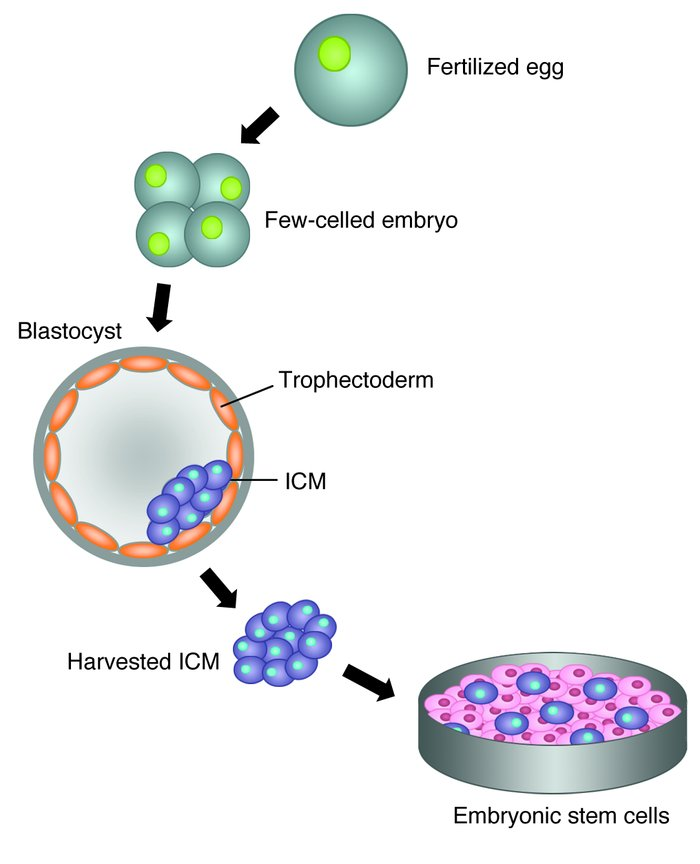
\includegraphics[width=0.5\linewidth]{JCI0423065.f1.jpg}
        \end{tikzfigure}

        \begin{tikzfigure}[Induced Pluripotent Stem Cell Process]
            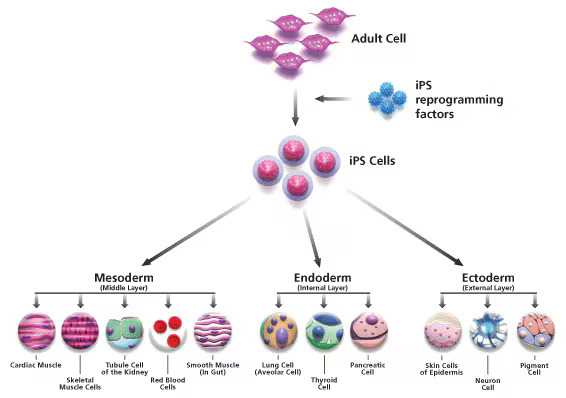
\includegraphics[width=0.7\linewidth]{ipsc-pathway.jpg}
        \end{tikzfigure}
        
    }

    \column{0.32}
    \block{Fetus Human Rights}{
        \begin{tikzfigure}[Unborn Human Fetus Compared to a Adult Human Hand \cite{a2024}]
            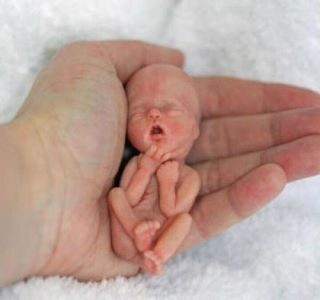
\includegraphics[width=0.7\linewidth]{1638394116879.jpeg}
        \end{tikzfigure}
        \textit{}{Response:} \\
        Senator, the answer to “Do human rights apply to the unborn?” is “Yes” and the
        evidence is incontrovertible. Any view to the contrary cannot have taken properly
        into account the definite rules and principles set down to resolve any doubts about
        meaning. The answer to this question must take full account of both 
        \begin{itemize}
            \item[(a)] the historical records of what was agreed in the seven Human Rights
            Conventions; and
            \item[(b)] the defining principles of human rights as set out in the Universal Declaration
            and codified in law in these Conventions.
        \end{itemize}
        Views are invalid if they contradict the historical facts
        \begin{itemize}
            \item that the Universal Declaration recognized the need for…special
            safeguards and care, including legal protection before as well as after
            birth.
            \item that \textbf{these rights belong to “all members of the human family”
             and
            especially to all children “without any exception whatsoever”
             and
            “without discrimination of any kind”}
            ; and 
            \item that the International Covenant on Civil and Political Rights confirms
            that for all members of the human family, every human being, 
            \cite{parliementofaustralia_do}
        \end{itemize}

        
    }
    
    \block{References}{
        \vspace{-1em}
        \begin{footnotesize}
        \printbibliography[heading=none]
        \end{footnotesize}
    }
\end{columns}
\end{document}